\begin{align}
Z-5x-3y=0\\
3x+5y+s_1=15\\
5x+2y+s_2=10
\end{align}
We will write the simplex tableau
\begin{align}
\myvec{
 x & y & s_1 & s_2 & c  \\ 
  3 & 5 & 1 & 0 & 15 \\ 
  \hlight{5} & 2 & 0 & 1 & 10  \\ \hline
  -5 & -3 & 0 & 0 & 0 
}
\end{align}
Keeping the pivot element as $5$, we will use gauss-jordan elimination.
\begin{align}
\myvec{
  x & y & s_1 & s_2 & c  \\[0.1cm] 
  0 & \hlight{\frac{19}{5}} & 1 & \frac{-3}{5} & 9 \\
  1 & \frac{2}{5} & 0 & \frac{1}{5} & 2  \\ \hline
  0 & -1 & 0 & 1 & 10 
}
\end{align}
Keeping the pivot element as $\frac{19}{5}$, we will use gauss-jordan elimination.
\begin{align}
\myvec{
  x & y & s_1 & s_2 & c  \\ 
  0 & 1 & \frac{5}{19} & \frac{-3}{19} & \frac{45}{19} \\ 
  1 & 0 & \frac{-2}{19} & \frac{5}{19} & \frac{20}{19}  \\ \hline 
  0 & 0 & \frac{5}{19} & \frac{16}{19} & \frac{235}{19} \\
}
\end{align}
In this tableau, there are no negative elements in the bottom row. We have therefore determined the optimal solution to be:
\begin{align}
(x,y,s_1,s_2)=\left(\frac{20}{19},\frac{45}{19},0,0\right)\\
Z=5x+3y\\
Z=5\times\frac{20}{19}+3\times\frac{45}{19}\\
Z=\frac{235}{19}
\end{align}
\begin{figure}[h]
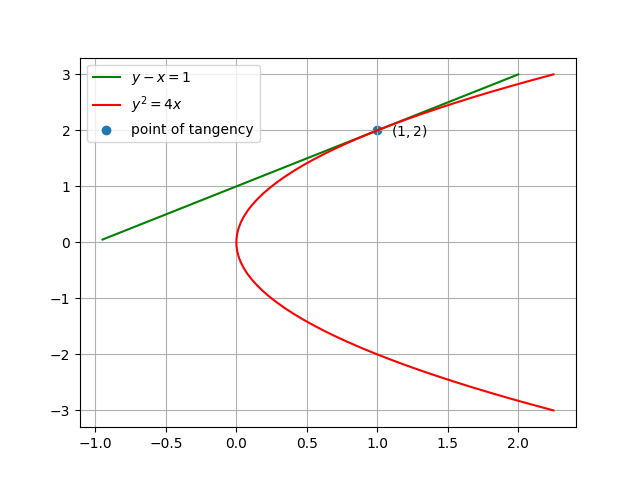
\includegraphics[width=\columnwidth]{./solutions/4/5/Figure_1.png}
\caption{optimal point through the intersection of various lines}
\label{fig:Figure_1}
\end{figure}
The given problem can be expressed in general as matrix inequality as:
%\begin{align}
%\max_{\vec{x}} Z &= \myvec{5 & 3}\vec{x}
%\\
%s.t. \quad 
%\myvec{
%3 & 5
%\\
%5 & 2
%}
%\vec{x} &\preceq \myvec{15\\10}
%\\
%\vec{x} &\succeq \vec{0}\\
%\vec{y} &\succeq \vec{0}
%\end{align}
\begin{align}
\max_{\vec{x}} &\vec{c}^{T}\vec{x}
\\
s.t. \quad \vec{A}\vec{x} &\le \vec{b},
\\
\vec{x} &\succeq\vec{0}\\
\vec{y} &\succeq \vec{0}
\end{align}
%
where
\begin{align}
\vec{c} &= \myvec{5 \\ 3}
\\
\vec{A} &=
\myvec{
3 & 5
\\
5 & 2
}
\\
\vec{b}&=\myvec{15\\10}
%
\end{align}
%
and can be solved using {\em cvxpy}. 
Hence,
\begin{align}
\vec{x} = \myvec{1.05263158\\2.36842105}, Z = 12.36842102
\end{align}

